\chapter{ نمونه‌هایی از قراردادن اشکال}
\label{chap:chap2}

در این قسمت، سعی کردم آنچه برای آوردن تصاویر لازم است را فراهم کنم. 
توجه داشته باشید که متداول است که یک پوشه برای عکس‌ها ساخته می‌شود تا فایل‌ها نظم و ترتیب بهتری داشته باشند. من در تهیه این قالب یک پوشه
\lr{'figs'}
درست کرده‌ام و همه عکس‌ها را در آن قرار داده‌ام. توجه داشته باشید که اسم و آدرس هر عکس است که در ترسیم آن مهم است.
آوردن تصویرهای تکی و شکل‌های دسته‌ای را جداگانه آورده‌ام.

\section{
شکل با یک تصویر تکی
}

شکل
\ref{fig:clock_tower_photo}
یک نمونه است. به اسکریپت مربوط به آن دقت کنید و سعی کنید معنی هر دستور را بفهمید تا بتوانید در صورت تمایل، در گزارش خودتان تغییرات لازم را ایجاد کنید. در غیر اینصورت، این یک نمونه عادی از آوردن شکل در متن است که می‌توانید مستقیما از آن استفاده کنید.

\begin{figure}[h]
    \centering
    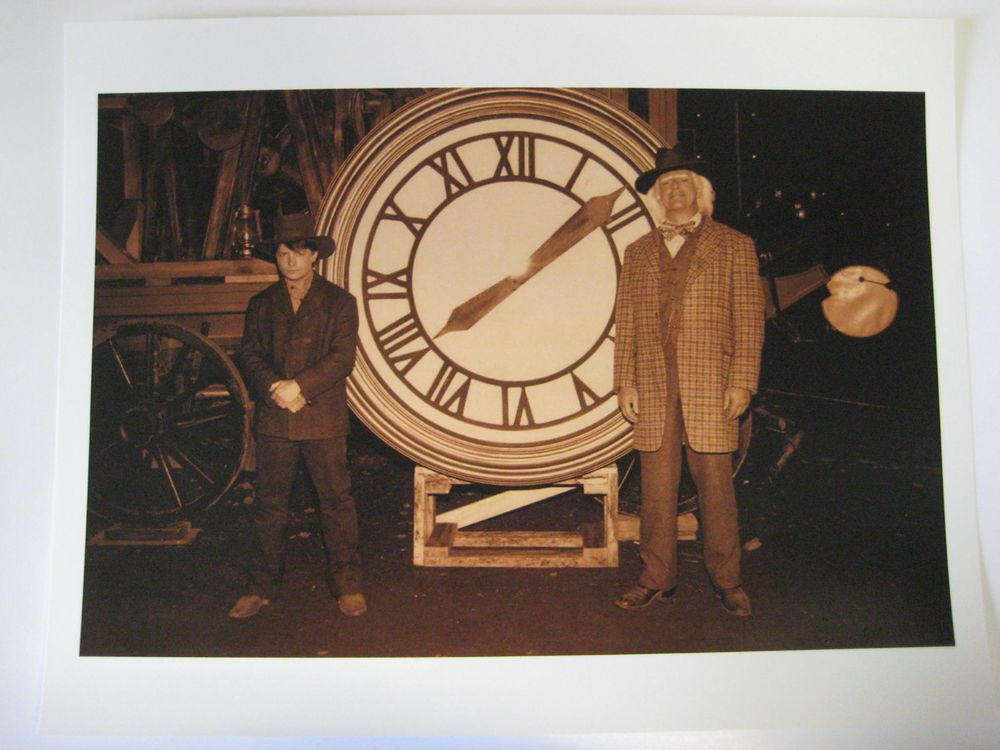
\includegraphics[width=0.5\textwidth]{figs/doc_and_marty.jpg}
    \caption{
    توضیح زیر عکس
    }
    \label{fig:clock_tower_photo}
\end{figure}


\section{
شکل با چند عکس داخل آن
}


یک نمونه از تصویر با چند عکس داخل آن:


\begin{figure}[h]
\centering
\subfigure[نمای آغاز]{
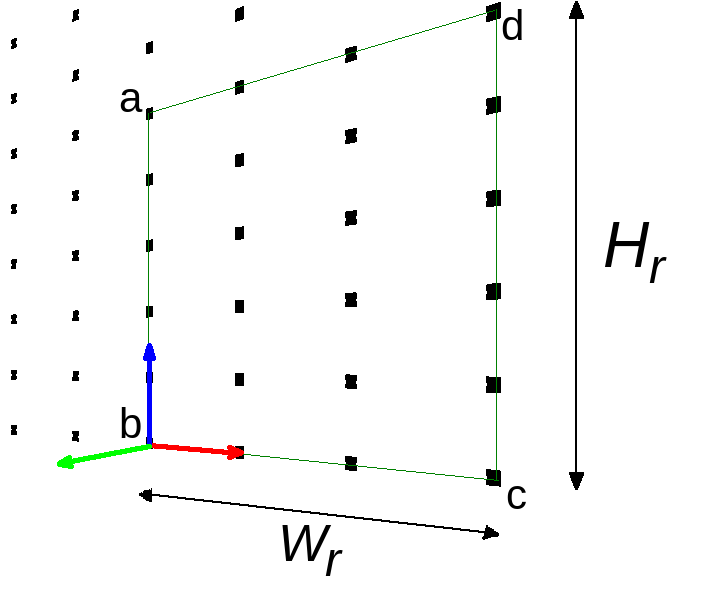
\includegraphics[width=0.3\linewidth]{figs/poor_view.png}
	\label{fig:poor_view}
}
\hspace*{15mm}
\subfigure[نمای پایان]{
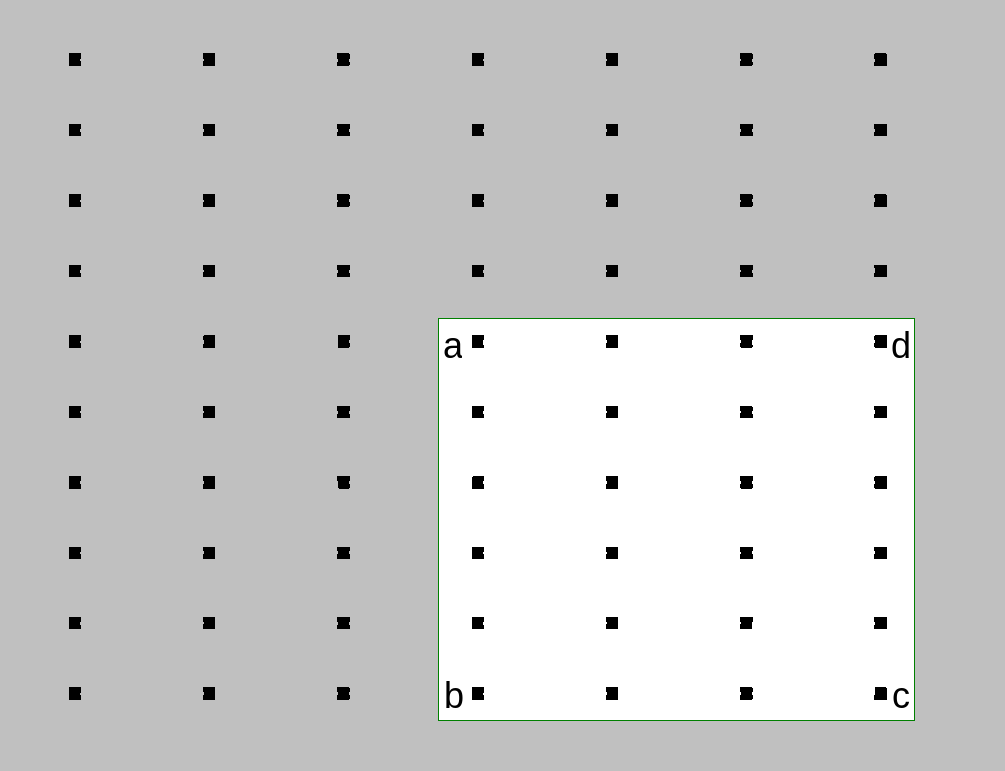
\includegraphics[width=0.3\linewidth]{figs/exact_view.png}
	\label{fig:exact_view}
}

\caption{نمای دوربین ریزپرنده در آغاز و پایان مرحله بهینه‌سازی موقعیت دید}

\label{fig:g1_views}
\end{figure}

یک نمونه دیگر با تعداد عکس بیشتر:

\begin{figure}[ht]
\centering
\subfigure[]{
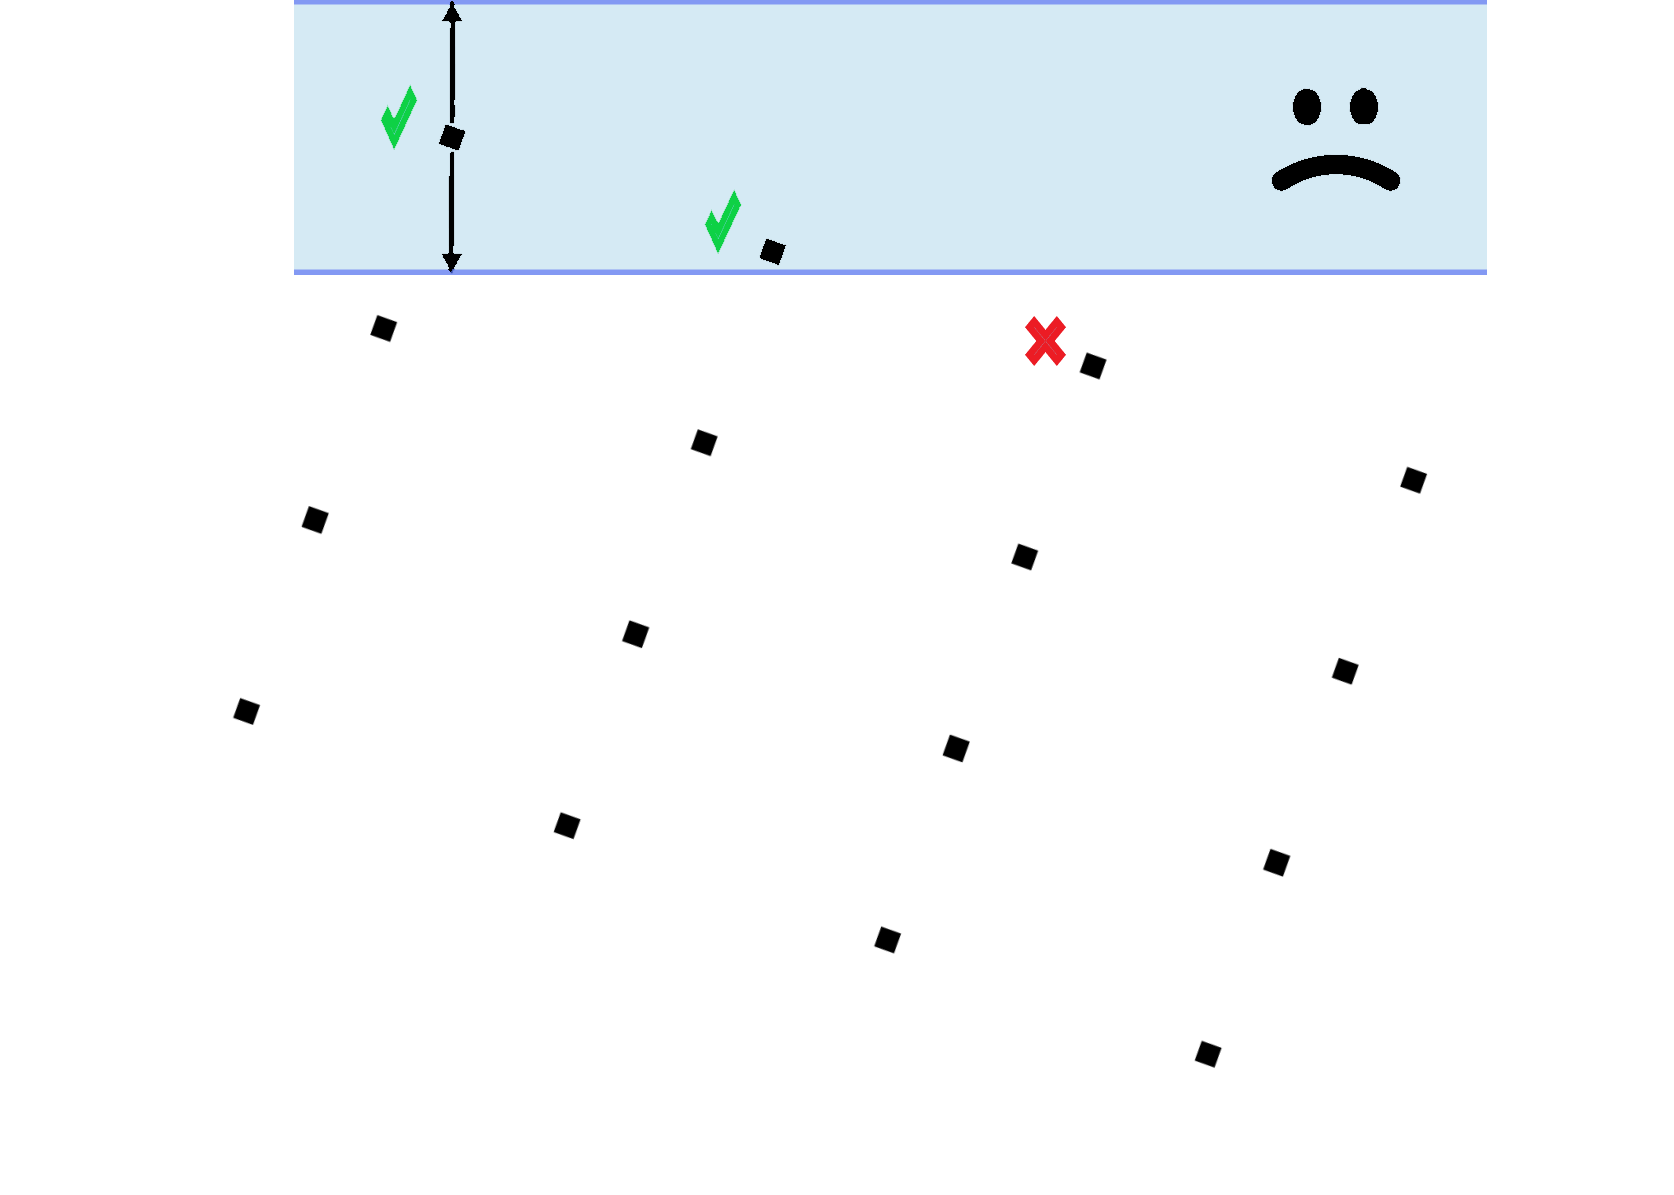
\includegraphics[width=0.3\linewidth]{figs/algorithm1.png}
	\label{fig:sc_vis_algorithm1}
}
\hspace*{1mm}
\subfigure[]{
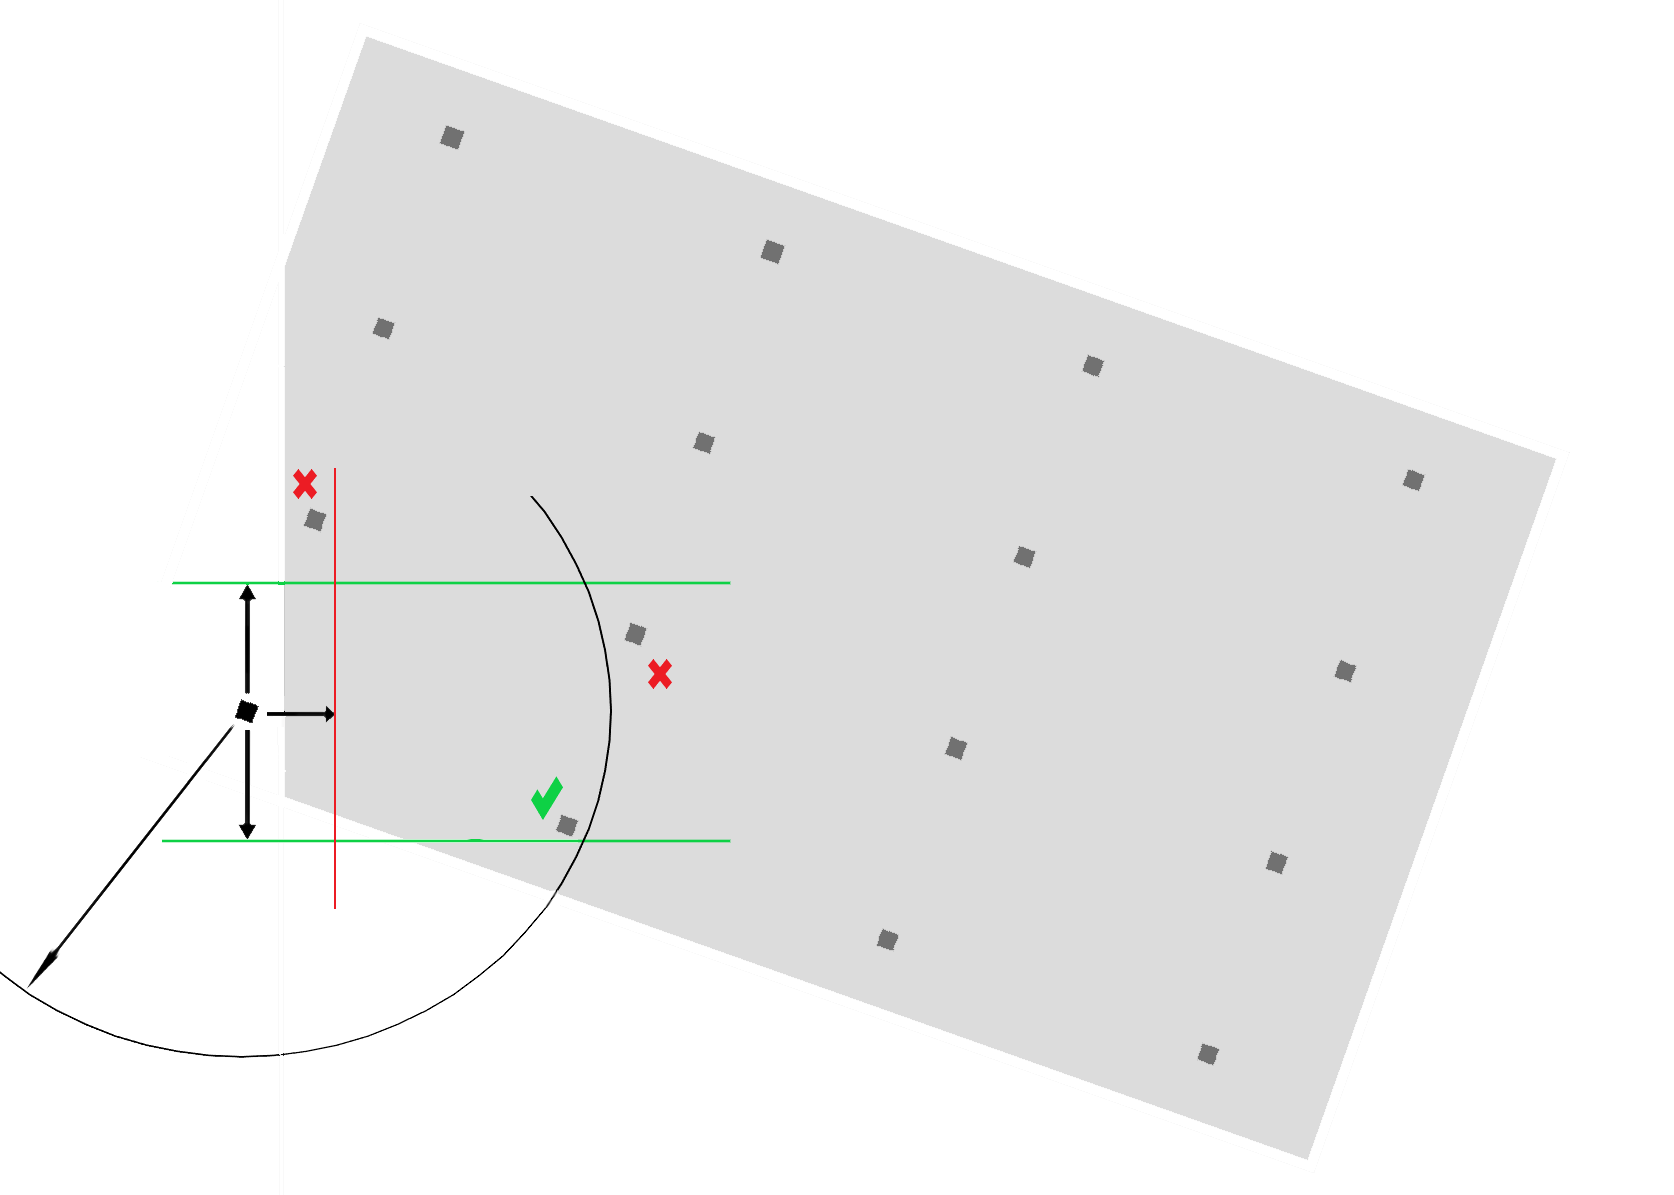
\includegraphics[width=0.3\linewidth]{figs/algorithm2.png}
	\label{fig:sc_vis_algorithm2}
}
\hspace*{1mm}
\subfigure[]{
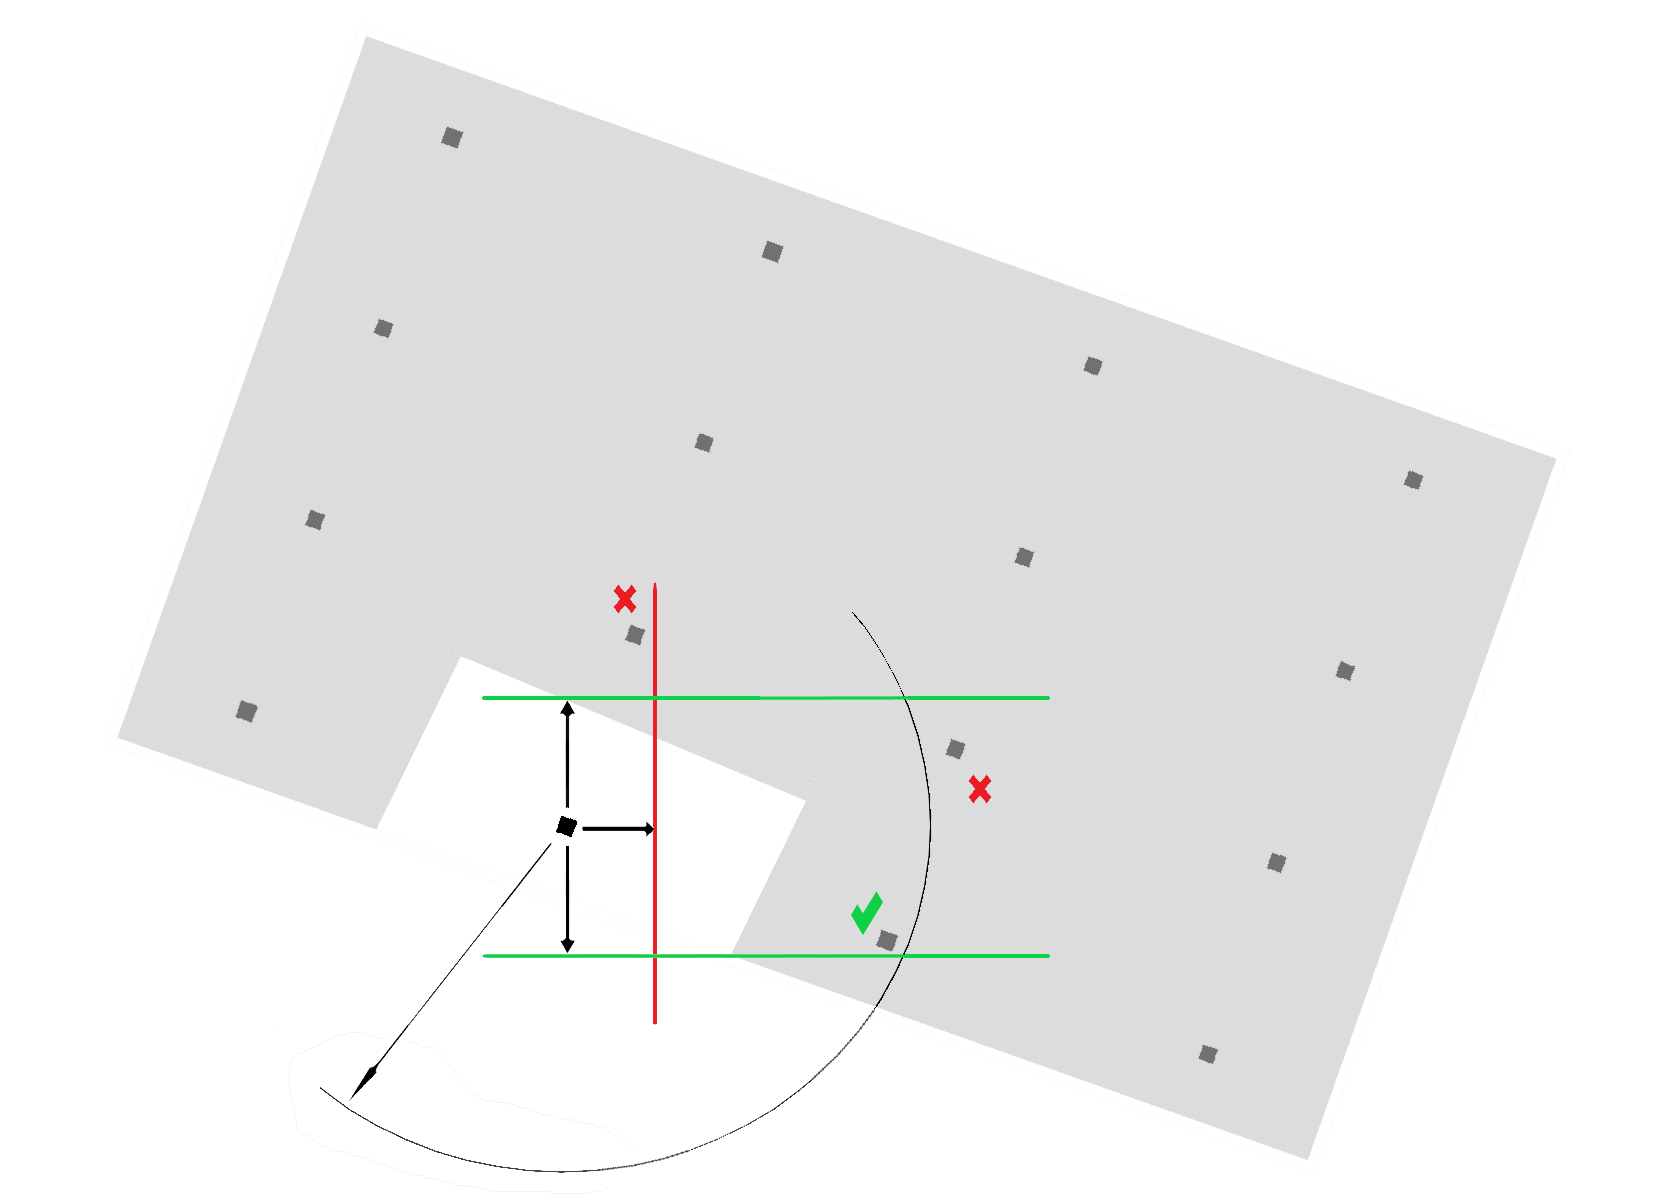
\includegraphics[width=0.3\linewidth]{figs/algorithm3.png}
	\label{fig:sc_vis_algorithm3}
}
\hspace*{1mm}
\subfigure[]{
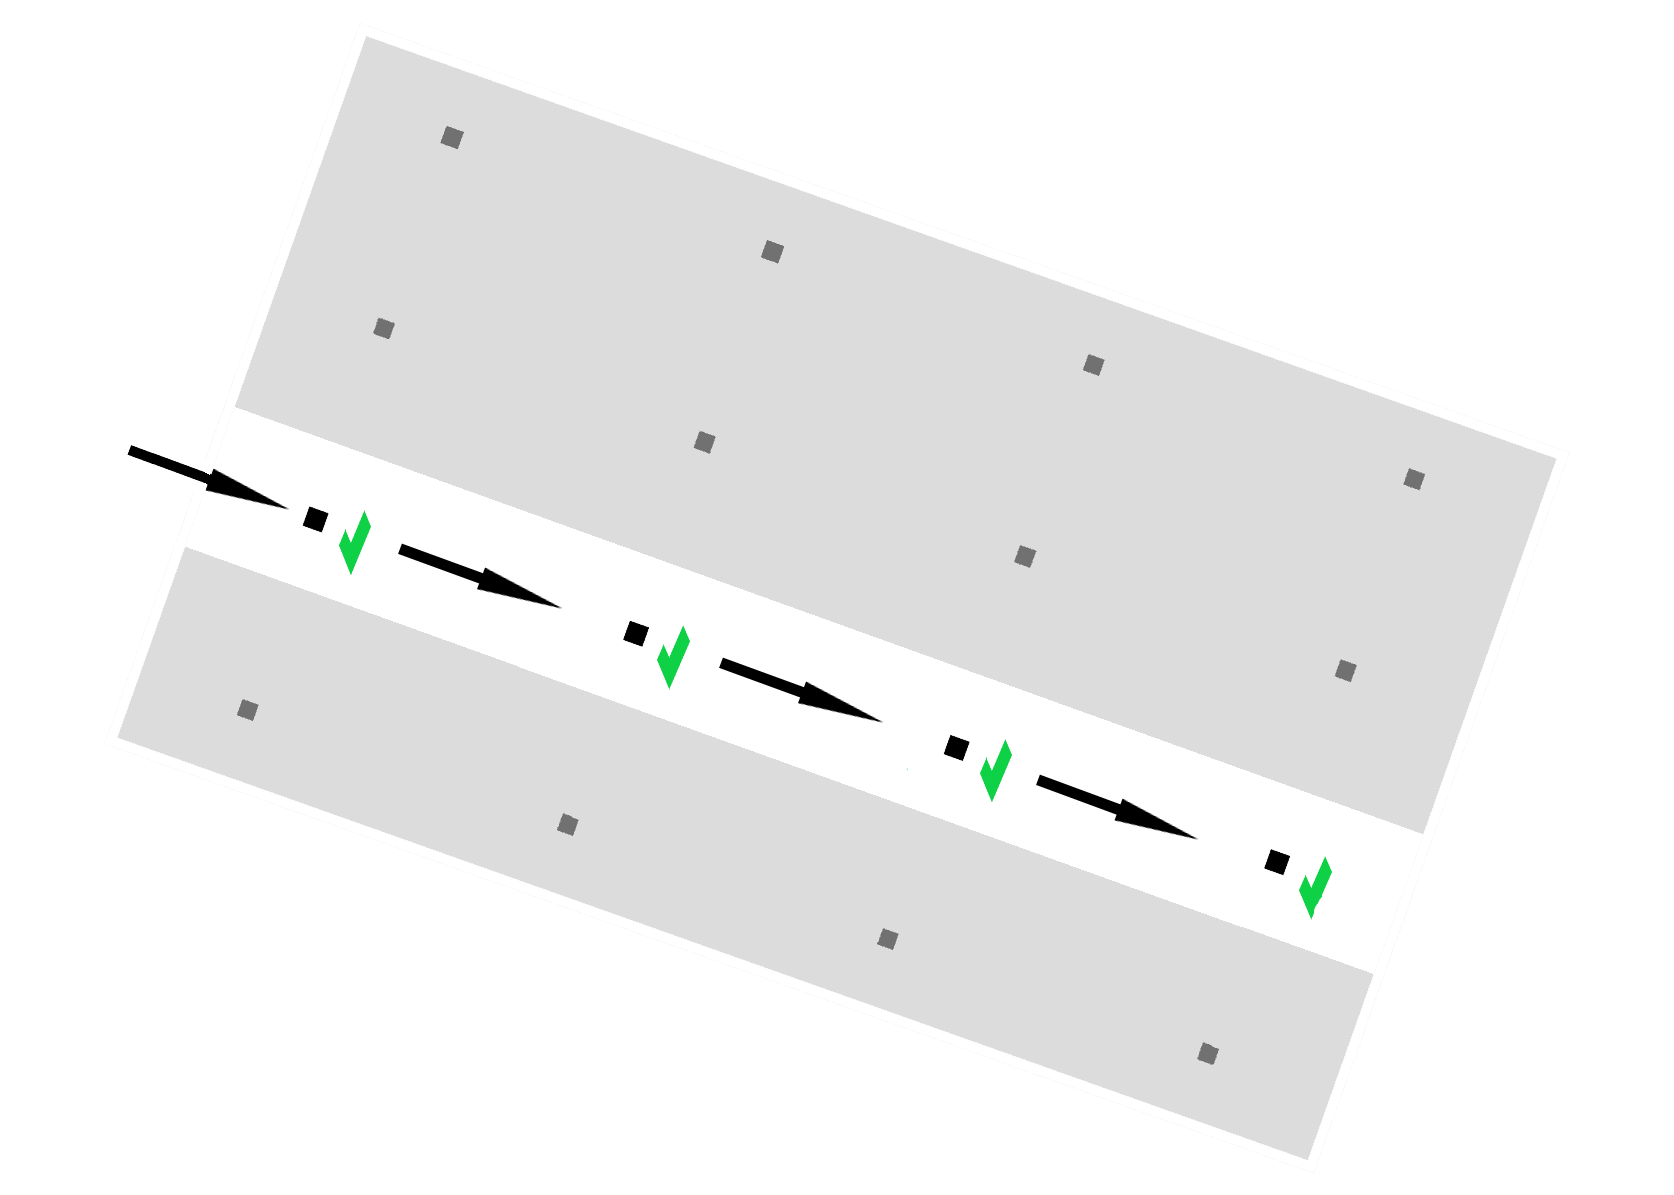
\includegraphics[width=0.3\linewidth]{figs/algorithm4.png}
	\label{fig:sc_vis_algorithm4}
}
\hspace*{1mm}
\subfigure[]{
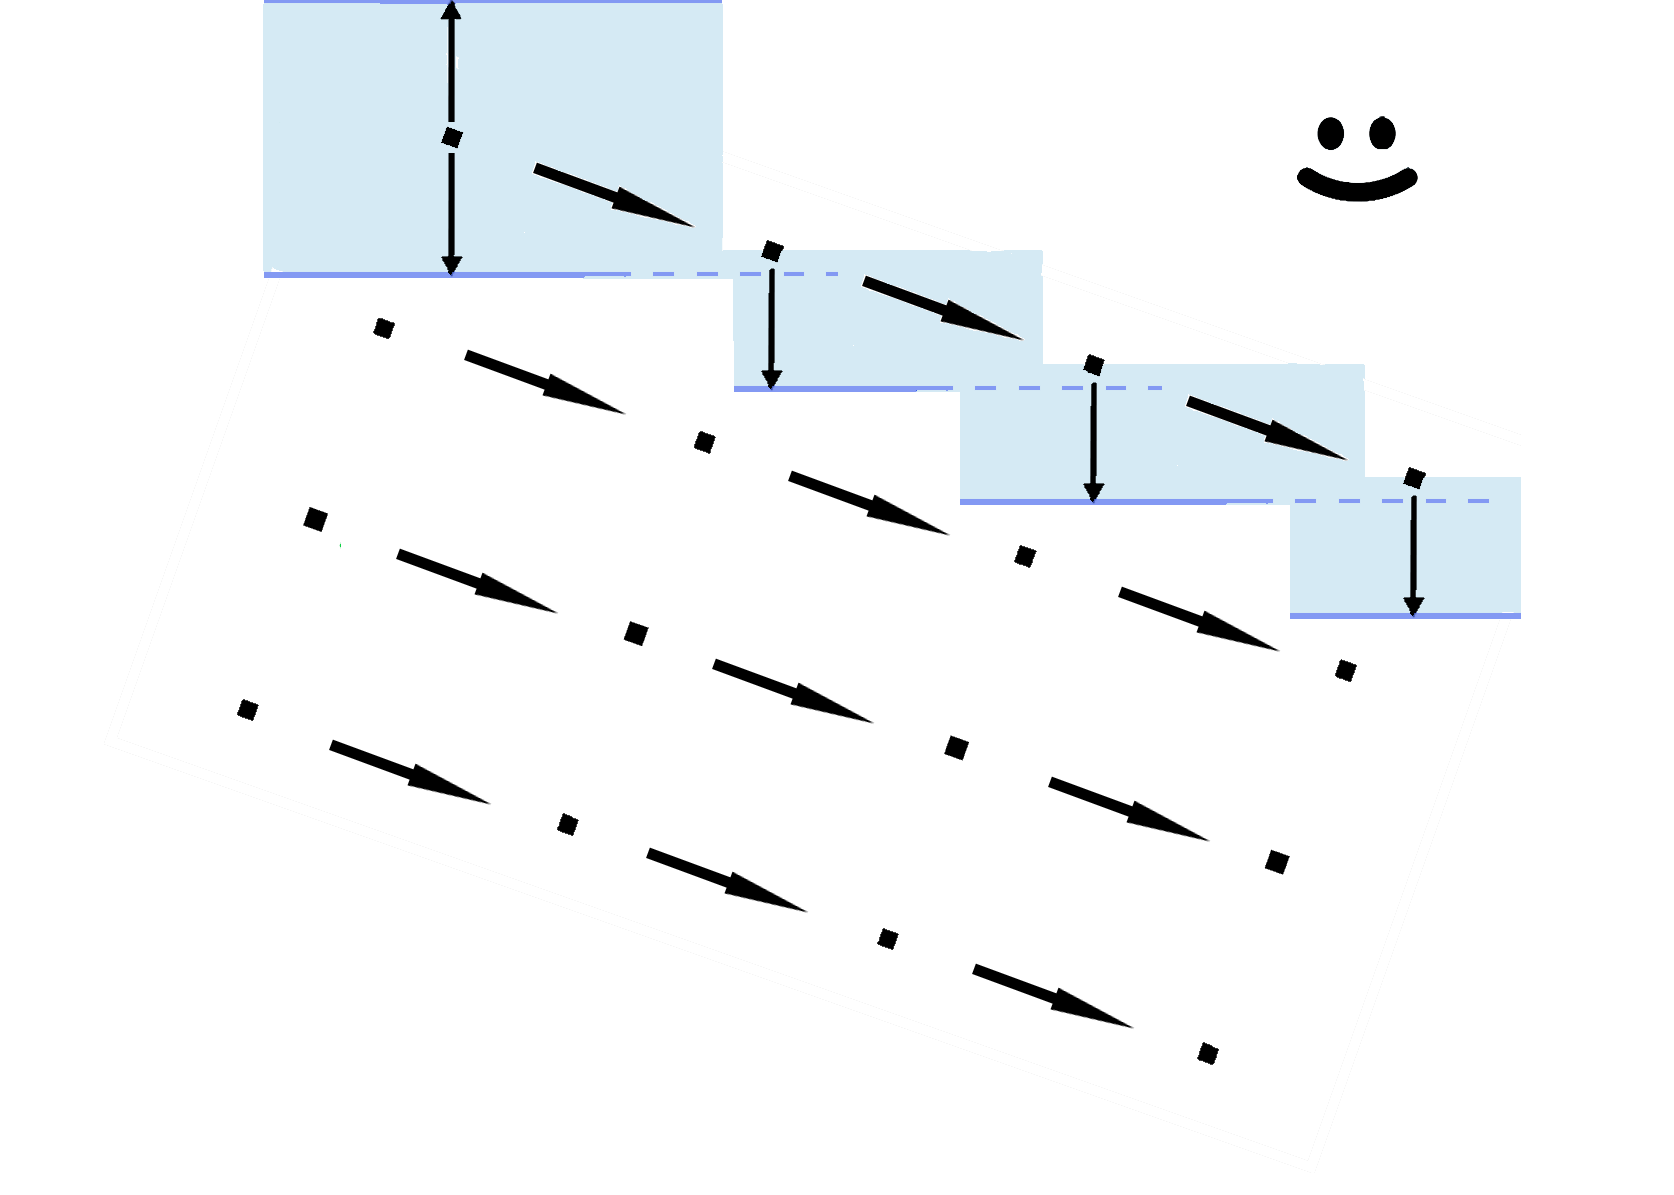
\includegraphics[width=0.3\linewidth]{figs/algorithm5.png}
	\label{fig:sc_vis_algorithm5}
}

\caption{
نمایی از مراحل پردازش داده جدول نقاط در روش دسته‌بندی پله‌ای
}
\label{fig:sc_algorithm}
\end{figure}